\documentclass{article}
\usepackage[a4paper, margin=0.5in]{geometry}
\usepackage[utf8]{inputenc}
\usepackage{amsmath}
\usepackage{stmaryrd}
\usepackage{graphicx}

\renewcommand\t[1]{\text{#1}}
\renewcommand\d{\text{ . }}
\newcommand\lwt[1]{$_\text{#1}$}

\usepackage{graphicx}

\begin{document}

% \maketitle

\section{}

\subsection*{a}

$$\llbracket \text{every wizard but Harry} \rrbracket^M = \{P \subseteq U_M | \llbracket \text{wizard} \rrbracket \subseteq P \wedge \llbracket \text{harry} \rrbracket \not\subset P\}$$
$$\llbracket\text{fear Voldemort}\rrbracket^M \in \llbracket\text{every wizard but Harry}\rrbracket^M$$


\subsection*{b}

$$\llbracket \text{some but not all muggles} \rrbracket^M = \{P \subseteq U_M |  \text{card}(\llbracket\text{muggle}\rrbracket \cap P) > 0 \wedge \llbracket\text{muggle}\rrbracket \cap P \neq \llbracket\text{muggle}\rrbracket\}$$
$$\llbracket\text{afraid of magic}\rrbracket^M \in \llbracket\text{some but all not muggles}\rrbracket^M \Leftrightarrow$$

\subsection*{c}

$$\llbracket \text{at most five girls} \rrbracket^M = \{P \subseteq U_M |  \text{card}(\llbracket\text{girl}\rrbracket \cap P) \leq 5\}$$
$$\llbracket\text{play quidditch}\rrbracket^M \in \llbracket\text{at most five girls}\rrbracket^M$$

\subsection*{d}

$$\llbracket \text{five Gryffindor} \rrbracket^M = \{P \subseteq U_M |  \leq \text{lower\_boundary\_few}(C) \leq  \text{card}(\llbracket\text{Gryffindor member}\rrbracket \cap P) \leq \text{upper\_boundary\_few}(C)\}$$
$$\llbracket\text{is lazy}\rrbracket^M \in \llbracket\text{five Gryffindor}\rrbracket^M$$

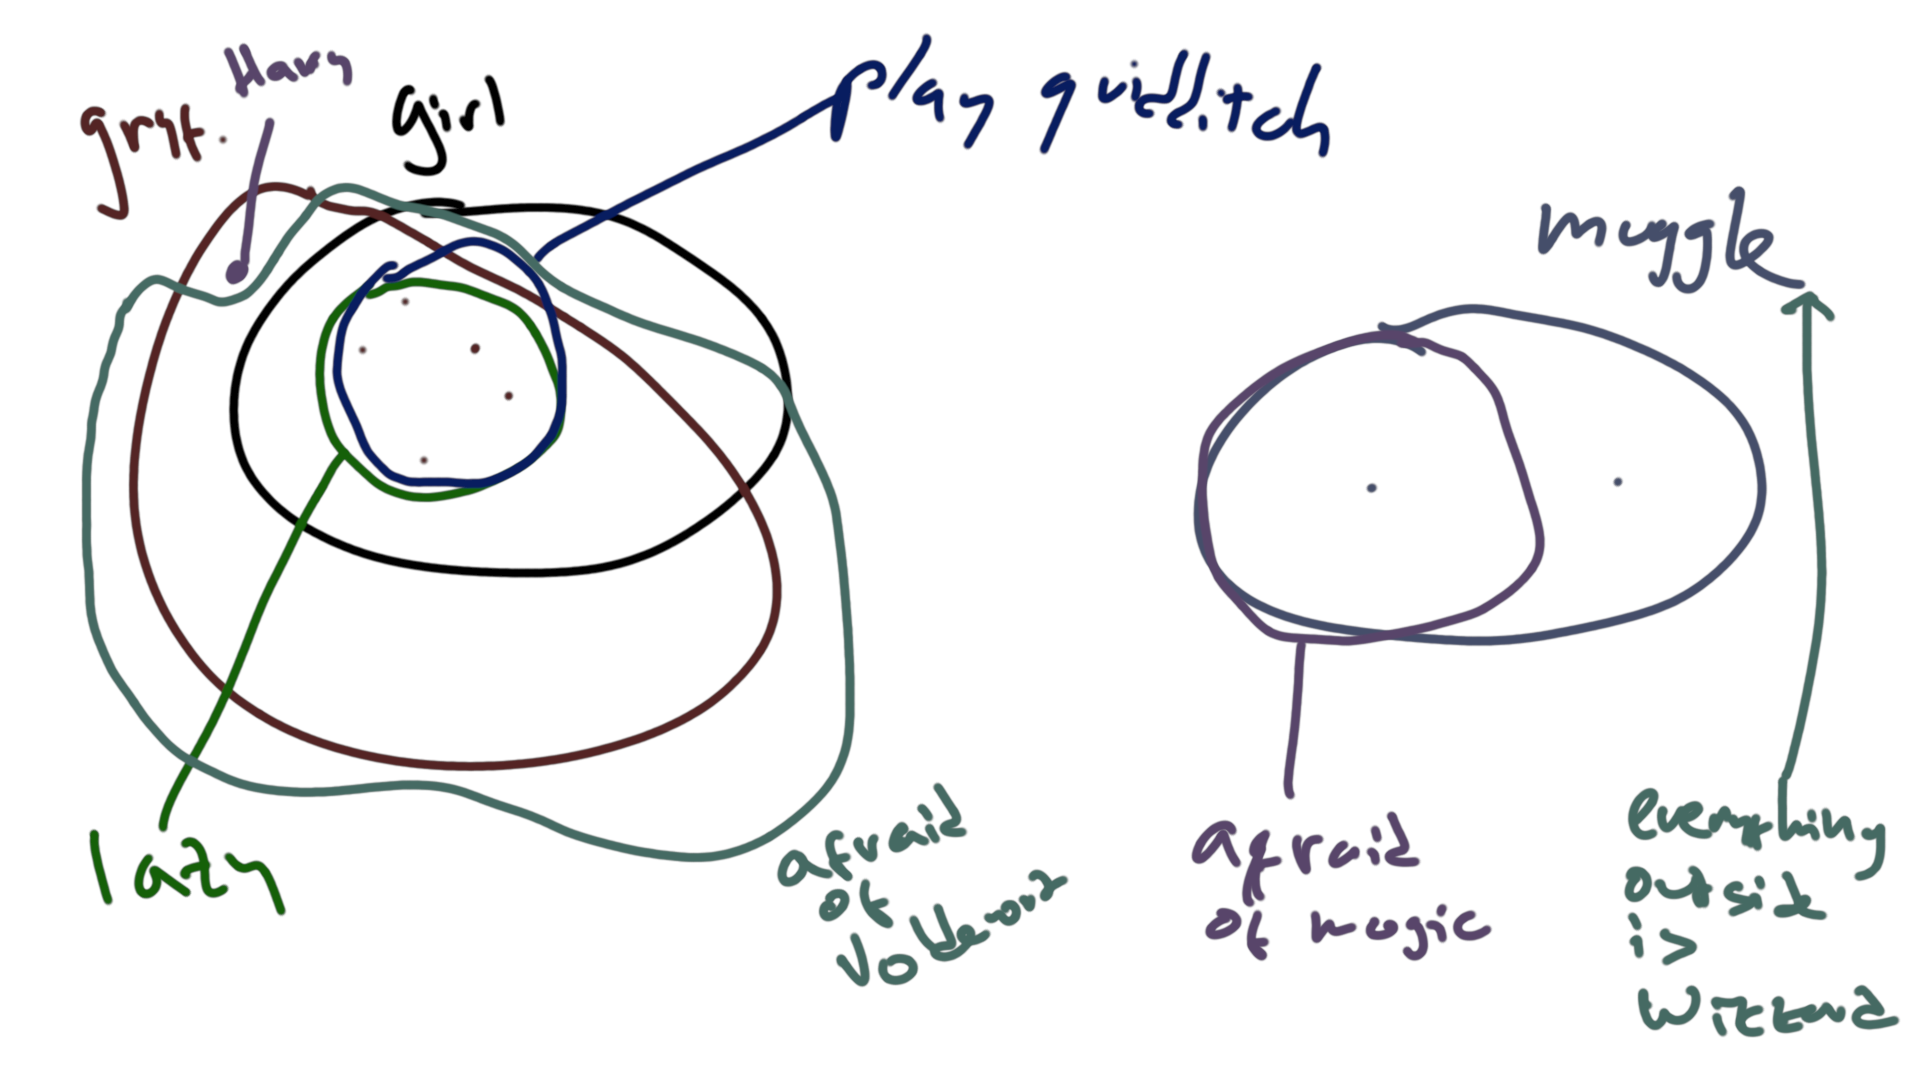
\includegraphics[width=\linewidth]{world.png}

\section{}

\subsection*{a}

\text{}

\textit{Some but not all} men \emph{walked rapidly}.
$\Rightarrow$
\textit{Some but not all} men \emph{walked}.
$\Rightarrow$
Left upward

\textit{Some but not all} \emph{men} walked.
$\Rightarrow$
\textit{Some but not all} \emph{humans} walked.
$\Rightarrow$
Right upward (persistent)

\subsection*{b}

\text{}

\textit{At most five} men \underline{walked}.
$\Rightarrow$
\textit{At most five} men \underline{walked rapidly}.
$\Rightarrow$
Left downward

\textit{At most five} \underline{humans} walked.
$\Rightarrow$
\textit{At most five} \underline{men} walked.
$\Rightarrow$
Right downward (antipersistent)

\subsection*{c}

\text{}

\textit{Exactly five} men \underline{walked}.
$\Rightarrow$
\textit{Exactly five} men \underline{walked rapidly}.
$\Rightarrow$
Left downward

(\textit{Exactly five} \underline{men} walked.
$\not\Rightarrow$
\textit{Exactly five} \underline{humans} walked.)$\wedge$(\textit{Exactly five} \underline{humans} walked.
$\not\Rightarrow$
\textit{Exactly five} \underline{men} walked.)

$\Rightarrow$
Right non-monotonous

\section{}

\text{}

Let $Q$ be an upward monotonous quantifier. Therefore:

$$\forall X, Y: X \in Q \wedge X \subseteq Y \Rightarrow Y \in Q$$

Then the following $P$: holds:

$$\forall X', Y': X' \not\in Q \wedge X' \subseteq Y' \Rightarrow Y' \not\in Q$$

For contradiction assume that it is not the case, therefore:

$$\forall X', Y': X' \not\in Q \wedge X' \subseteq Y' \wedge Y' \in Q$$

Which is in contradiction with the premise if we substitute $X=Y'$ and $Y'=X$.

Since $Y\in Q \Leftrightarrow Y \not\in \neg Q$. The statement $P$ can therefore be rewritten as:

$$\forall X', Y': X' \in \neg Q \wedge X' \subseteq Y' \wedge Y' \in \neg Q$$


Which describes the downward monotonicity of $\neg Q$

\end{document}

